\documentclass[a4paper]{article}

\usepackage[utf8]{inputenc}
\usepackage{listings}
\usepackage{url}
\usepackage{graphicx}
\usepackage{authblk}
\usepackage{xspace}
\usepackage{tabularx}
\usepackage{verbatim}

\newcommand{\code}[1]{\\ \\ \texttt{#1} \\ \\ }


\title{Building DPF releases}


\begin{document}

\maketitle

\section{Tycho and the DPF build system}

The DPF project uses a build system based on Maven and Tycho plugin. This allows us to build, test and package all the plugins belonging to the DPF
project using a single command. Furthermore, using a well supported build system allows the implementation of continuous integration solutions.
In this document I will treat Mavn as a commend line tool, however it is also possiblities to integrate Maven with Eclipse.

\subsection{Installing Dependencies}

The only technology required to build DPF is Maven. Maven will, based on the pom.xml files in the DPF plugins, automatically download
any other requirements. Instructions on how to install and use maven are availbale at \url{http://maven.apache.org/guides/getting-started/maven-in-five-minutes.html}. 

\subsection{Using maven with DPF}

Maven is controlled by pom.xml files. Each plugin as well as the root directory for the projects have one pom.xml file each. The pom.xml
file in the root directory has a list of the sub-projectst that are included in the build.

In order to use maven simply stand in the root directory and execute: \code{mvn [goal]} 
For instance, the command  to build, test and package the DPF build
is: \code{mvn install}
For more information on the goals that are available in Maven see \url{http://maven.apache.org/guides/introduction/introduction-to-the-lifecycle.html}.



%\begin{itemize}
%\item Why a build system
%\item Tycho and maven
%\item Intalling maven
%\item Uses of the build system
%\end{itemize}


\section{How build a release}

In order to build (compile) all the DPF plugins, stand in the root directory of the DPF repository and execute \code{mvn compile}. This will produce an
output with lines (among many others) similar to the ones shown in Fig.~\ref{fig:compile}. This output lists all the modules of the project wether the compilation was 
sucessfull. If one or more modules is not sucessfully compiles the output can be inspected to determine the cause of the compilation falioure. 

\begin{figure}
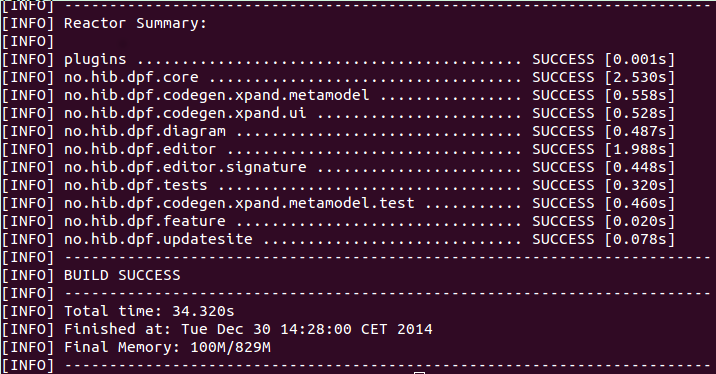
\includegraphics[width=\linewidth]{compile}

\caption{Output of the compile command}
\end{figure}

Testing a build can be done by executing: \code{mvn -fn check}
This will run all the test that are stored in test projects (See section~\ref{sec:plugins}).
This commands will produce an output similar to the one showed in Fig.~\ref{fig:compile}. However, the sucess of the test projects will depend on the resultes of the 
contained test cases. The results of the tests will also be stored in the target directory of each of the test projects. The \texttt{-fn} argument prevents maven from stopping at the first failiour it encounters so that all the tests are executed.

%\begin{itemize}
%\item Running tests
%\item Running builds
%\item Building fot other platforms
%\item The DPF Eclipse application
%\end{itemize}

\section{Adding a new plugin to the build}
\label{sec:plugins}

In order to add a new plugin to the build, first, the plugin is created as a regular eclipse plugin. Additionally, a pom.xml file must be added to the root directory
of the new plugin. A sample pom.xml is seen in listing~\ref{lst:pom}.

\begin{figure}
\begin{lstlisting}[caption={Sample pom.xml}]
<?xml version="1.0" encoding="UTF-8"?>
<project 
  xsi:schemaLocation="http://maven.apache.org/POM/4.0.0 
  http://maven.apache.org/xsd/maven-4.0.0.xsd" 
  xmlns="http://maven.apache.org/POM/4.0.0"
    xmlns:xsi="http://www.w3.org/2001/XMLSchema-instance">
  <modelVersion>4.0.0</modelVersion>
  <parent>
    <groupId>no.hib.dpf</groupId>
    <artifactId>plugins</artifactId>
    <version>0.0.1-SNAPSHOT</version>
  </parent>
  <groupId>no.hib.dpf</groupId>
  <artifactId>no.hib.dpf.YOUR_PLUGINID</artifactId>
  <version>0.1.1-SNAPSHOT</version>
  <packaging>eclipse-plugin</packaging>
</project>
\end{lstlisting}
\end{figure}

The <packaging> tag describes the type of the plugin. For a regulat eclipse plugin the value of this tag should be \texttt{eclipse-plugin}. For a test project
the value should be \texttt{eclipse-test-plugin}


In order to add the new plugin to the build it must be registered in the project pom.xml. This is done by adding a module tag inside the moduels tag that contains
the path to the module to  the project pom.xml file.

%\begin{itemize}
% \item creating a new pom.xml
% \item Adding the new plugin to the project build
%\end{itemize}


\end{document}
